% Drawing 154/06-9 -- folder 154, batch 06, archive page 112 (PDF page 113).
% Transcription: à gauche, deux dessins en couleur : deux droites orange $D_1$, $D_2$ qui se croisent en $s$, une courbe vert foncé qui les enjambe au-dessus d'une droite vert clair et d'une droite en tirets, des hachures et des flèches au crayon ; étiquettes $D_1$, $D_2$, en bas « $D_2$ », « $D_4$ » (\uncertain{lus}), et dans le second $D$, $D'$, $D'_1$, et une accolade marquée $\Delta_D$ ; en marge, « $\Delta_{D'}$ »
% Kind: two crossing lines straddled by a dark green curve (two drawings). Method 2 (schematic redraw from the facsimile). Status: ok.
% Notes: Left, two colour drawings: two orange lines D_1, D_2 crossing at s, a dark green curve straddling them above a light green line and a dashed line (two dashed lines in fact: one along the curve, one under the light green line), pencil hatching (left out) and arrows; labels D_1, D_2 at the top, « D_2 », « D_4 » at the bottom (as read in the transcription), and in the second D, D', D'_1 and a brace marked Delta_D; in the margin « Delta_{D'} ». The two disks at the foot of the page are not covered by this mark nor by 06-10. Read from the page view.
% Coordinates: 1 unit = 1 mm = 1/100 of the crop width (bbox in page fractions: [0.116, 0.069, 0.375, 0.303]).
% Redrawn by Claude (claude-opus-5-5), issue #73, 2026-11-07; not checked by a human; not compiled (no TeX in the session).
% Revised by Claude (claude-opus-5-5) 2026-11-09 (issue #128) after Michel's check: vertices snapped to exact intersections (drawn points on their lines, meeting ends on the stroke they meet, near-concurrent lines through one computed point, curve ends on their rim); labels at \small as in folder 80 batch 3. Status: ok.
% Rights: reproduces part of the work -- behind RENDER_TRANSCRIPTS, never published by itself.
\documentclass[tikz,border=3pt]{standalone}
\usepackage{amsmath,amssymb}
\usetikzlibrary{patterns,arrows.meta}
\tikzset{Or/.style={orange!90!black}, Ye/.style={yellow!80!orange}, Lg/.style={green!60!black!70}, Dg/.style={green!45!black}, Br/.style={brown!80!black}, Rd/.style={red!85!black}, Bl/.style={blue!70!black}, Gy/.style={black!40}, pencil/.style={black!45}, struck/.style={black!35}, mark/.style={circle,draw,inner sep=1.3pt}, pt/.style={circle,fill,inner sep=0.9pt}, opt/.style={circle,draw,fill=white,inner sep=1.1pt}}
\colorlet{Or}{orange!90!black}\colorlet{Ye}{yellow!80!orange}\colorlet{Lg}{green!60!black!70}\colorlet{Dg}{green!45!black}\colorlet{Br}{brown!80!black}\colorlet{Rd}{red!85!black}\colorlet{Bl}{blue!70!black}\colorlet{Gy}{black!40}
\begin{document}
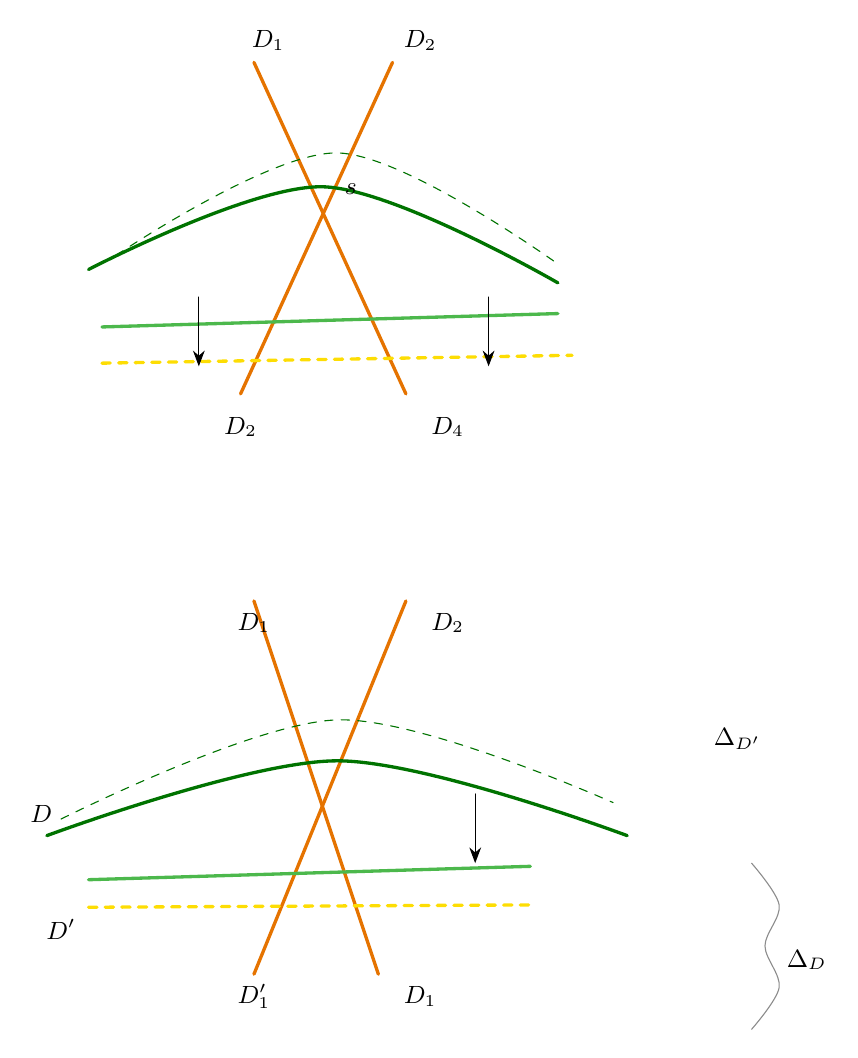
\begin{tikzpicture}[x=1mm,y=1mm,line cap=round,line join=round,font=\scriptsize]
\draw[Or,very thick] (29.8,-5.3) -- (49.1,-47.4);
\draw[Or,very thick] (47.4,-5.3) -- (28.1,-47.4);
\draw[Dg,very thick] plot[smooth, tension=0.55] coordinates {(8.8,-31.6) (38.6,-21.1) (68.4,-33.3)};
\draw[Dg,dashed] plot[smooth, tension=0.55] coordinates {(12.3,-29.8) (40.4,-16.8) (68.4,-30.9)};
\draw[Lg,very thick] (10.5,-38.9) -- (68.4,-37.2);
\draw[Ye,dashed,very thick] (10.5,-43.5) -- (70.2,-42.5);
\draw[-{Stealth[length=2mm]}] (22.8,-35.1) -- (22.8,-43.9);
\draw[-{Stealth[length=2mm]}] (59.6,-35.1) -- (59.6,-43.9);
\node[inner sep=1pt] at (42.1,-21.4) {\small $s$};
\node[inner sep=1pt] at (31.6,-2.5) {\small $D_1$};
\node[inner sep=1pt] at (50.9,-2.5) {\small $D_2$};
\node[inner sep=1pt] at (28.1,-51.6) {\small $D_2$};
\node[inner sep=1pt] at (54.4,-51.6) {\small $D_4$};
\draw[Or,very thick] (29.8,-121.1) -- (49.1,-73.7);
\draw[Or,very thick] (29.8,-73.7) -- (45.6,-121.1);
\draw[Dg,very thick] plot[smooth, tension=0.55] coordinates {(3.5,-103.5) (40.4,-94) (77.2,-103.5)};
\draw[Dg,dashed] plot[smooth, tension=0.55] coordinates {(5.3,-101.4) (40.4,-88.8) (75.4,-99.3)};
\draw[Lg,very thick] (8.8,-109.1) -- (64.9,-107.4);
\draw[Ye,dashed,very thick] (8.8,-112.6) -- (64.9,-112.3);
\draw[-{Stealth[length=2mm]}] (57.9,-98.2) -- (57.9,-107);
\node[inner sep=1pt] at (29.8,-76.5) {\small $D_1$};
\node[inner sep=1pt] at (54.4,-76.5) {\small $D_2$};
\node[inner sep=1pt] at (2.8,-100.7) {\small $D$};
\node[inner sep=1pt] at (5.3,-115.4) {\small $D'$};
\node[inner sep=1pt] at (29.8,-123.9) {\small $D'_1$};
\node[inner sep=1pt] at (50.9,-123.9) {\small $D_1$};
\draw[pencil] plot[smooth, tension=0.55] coordinates {(93,-107) (96.5,-112.3) (94.7,-117.5) (96.5,-122.8) (93,-128.1)};
\node[inner sep=1pt] at (100,-119.3) {\small $\Delta_D$};
\node[inner sep=1pt] at (91.2,-91.2) {\small $\Delta_{D'}$};
\end{tikzpicture}
\end{document}
